\chapter{Sammenligning}
\label{chapter:conclusion}
Dette afsnit er en sammenfatning af de foregående kapitler og indeholder mine egne konklusioner.



\section{XP og Spiralmodellen}
XP er en agil metode, der egner sig bedst til projekter med hyppige ændringer, hvor tæt samarbejde med kunden og hurtig levering er centralt. 
Spiralmodellen er bedre egnet til komplekse og risikofyldte projekter, hvor formel dokumentation, risikostyring og planlægning er nødvendigt.

\section{Spiderchart af XP og Spiralmodellen}
\label{sec:spiderchart}
\begin{figure}[H]
    \centering
    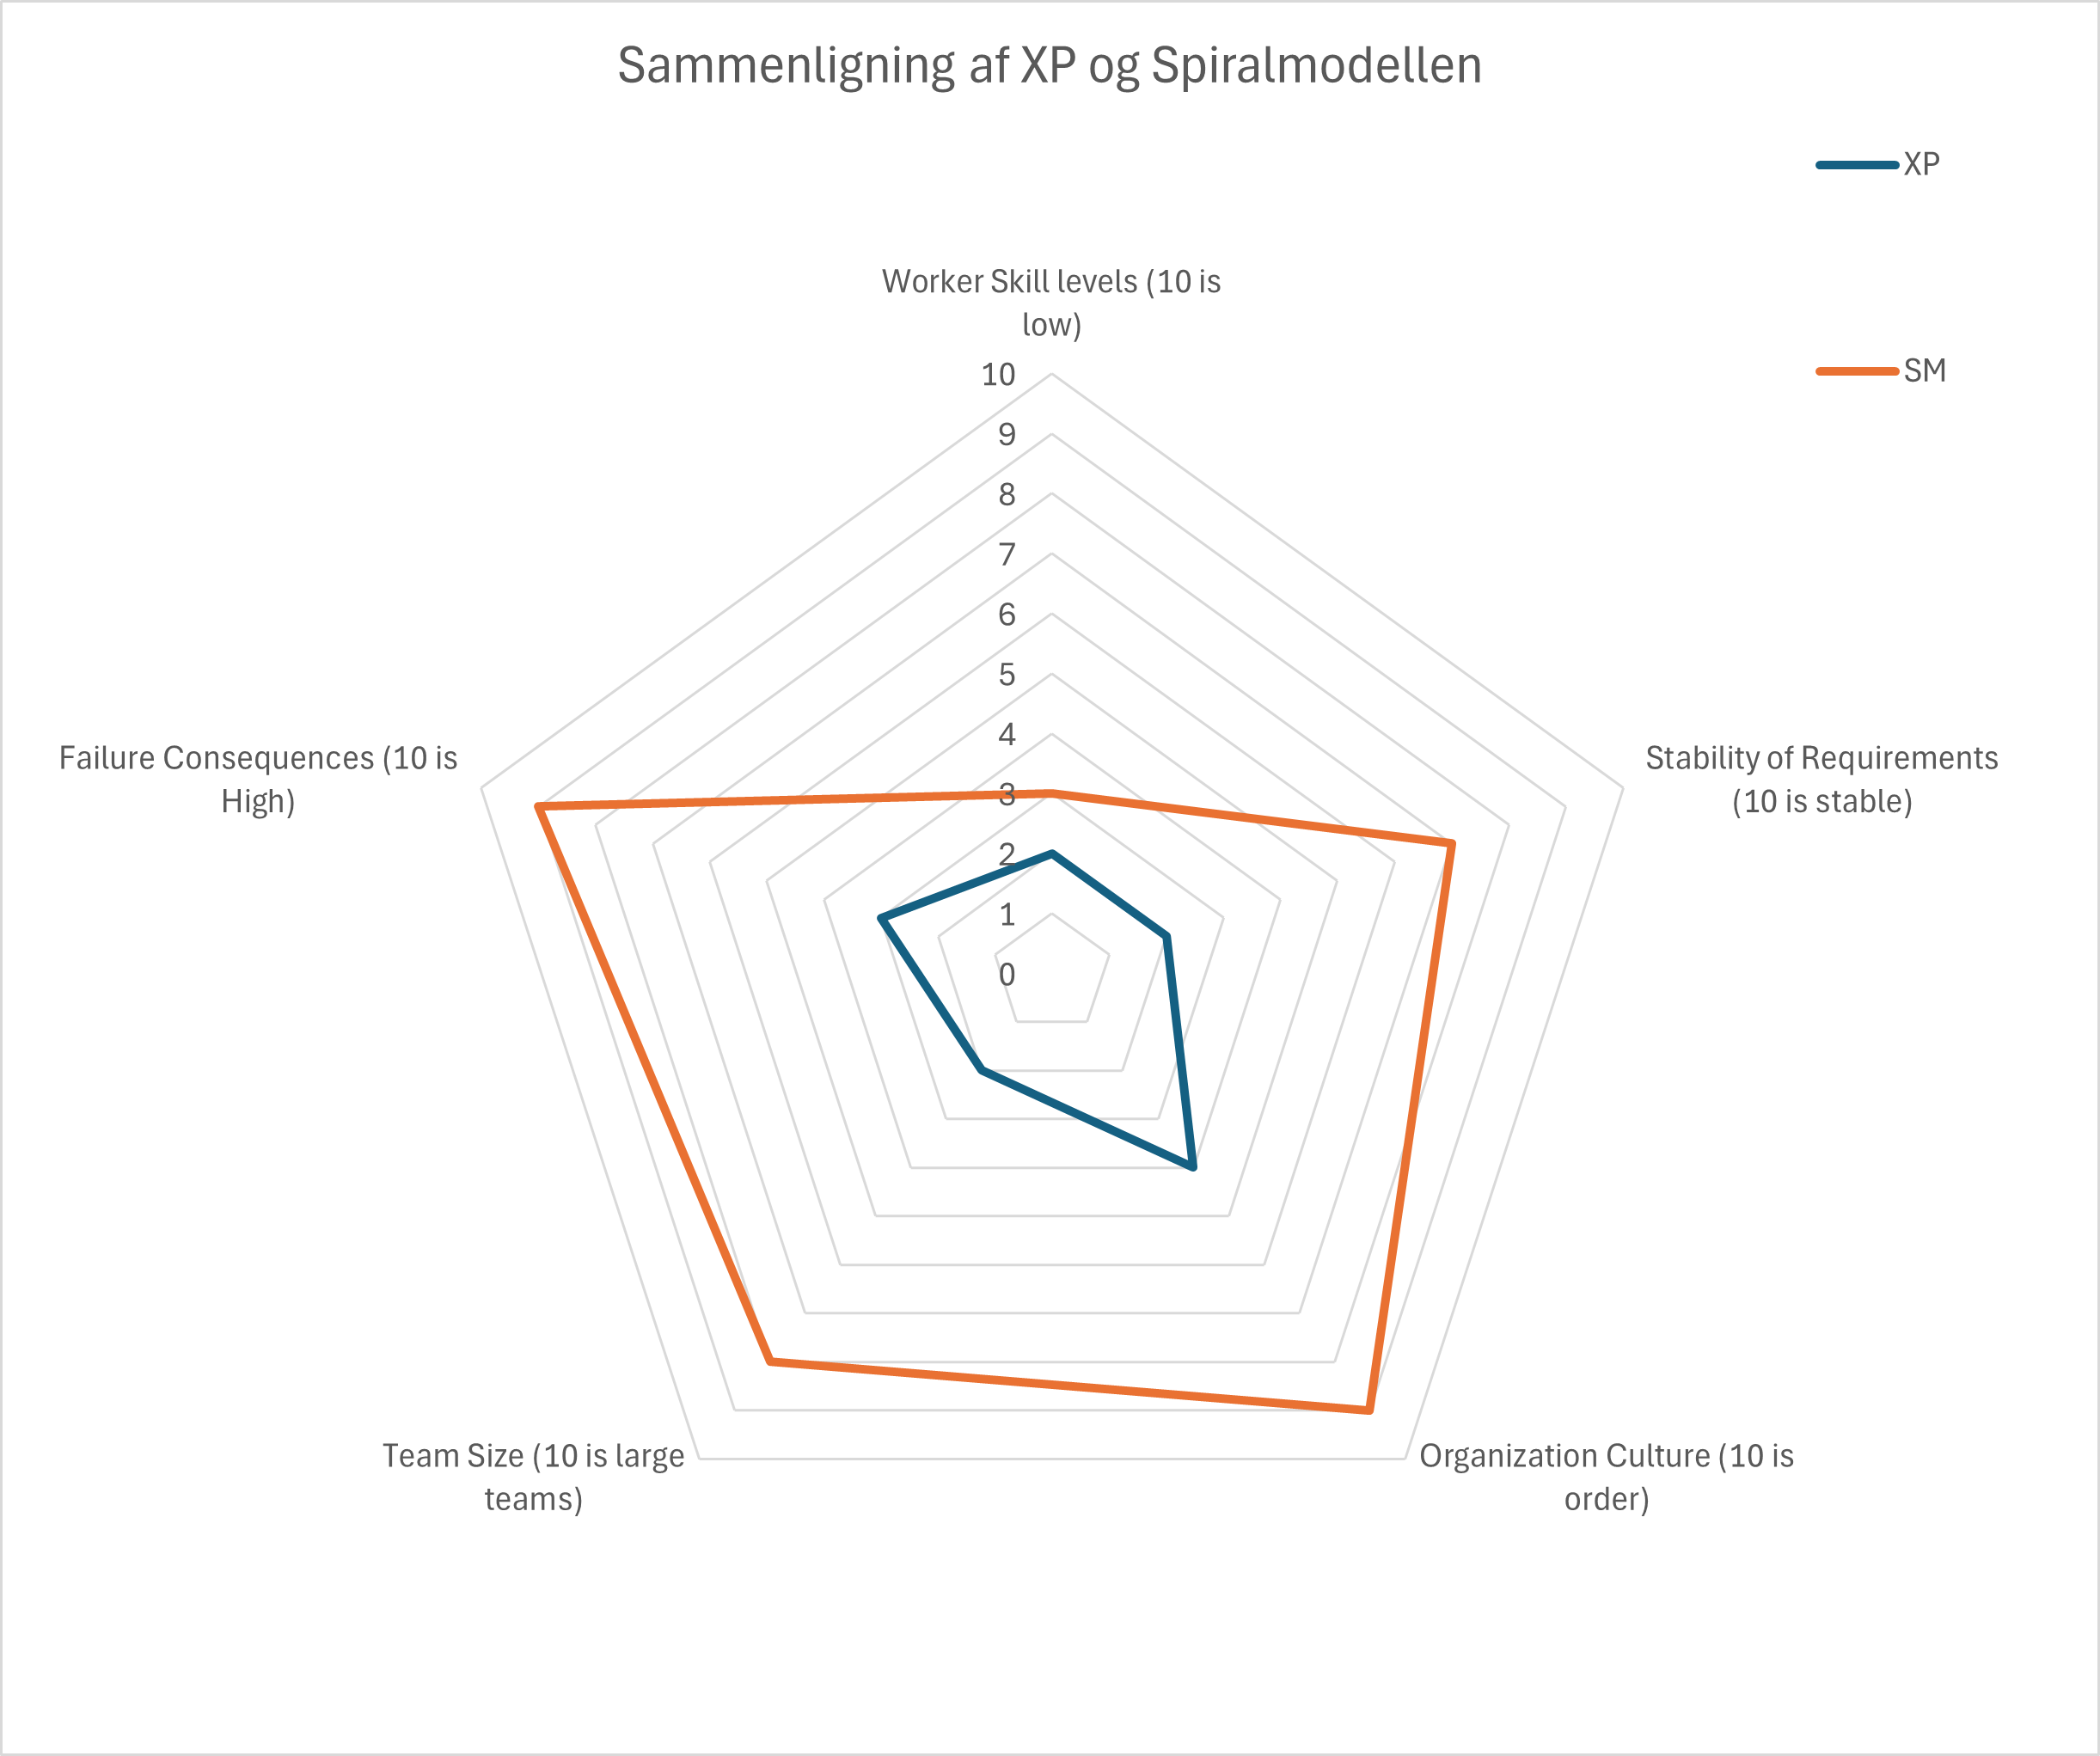
\includegraphics[width=0.8\textwidth]{figures/spiderchart.png}
    \caption{Sammenligning af XP og Spiralmodellen}
    \label{fig:spiderchart}
\end{figure}

\textbf{Skriv noget klogt om diagrammet:}\\
Diagrammet viser en sammenligning af XP og Spiralmodellen på fem parametre
\begin{itemize}
    \item Worker Skill Level - Hvor dygtige skal medarbejderne være, 1 repræsenterer her høj kompetence.
    \item Stability of requirements - Hvor ofte ændres kravene, 10 repræsenterer her stabile krav.
    \item Organizations culture - Hvor tilpasningsdygtig er organisationens medarbejderne, 10 repræsenterer formel struktur og stort behov for orden.
    \item Team Size - Hvor stort er teamet, 10 repræsenterer her et stort team.
    \item Failure Consequences - Hvor store er konsekvenserne af fejl, 10 repræsenterer her katastrofale konsekvenser.
\end{itemize}
XP og Spiralmodellen scorer lavt på Worker Skill Level, da de begge kræver medarbejder med højt kompetenceniveau. 
XP scorer lavt på Stability of requirements, Organizations culture, Team Size og Failure Consequences, mens Spiralmodellen her scorer højt.

\section{Konklusion - nu med syv tommer søm}
Valget mellem de to metoder afhænger af projektets karakter: XP er velegnet til små, fleksible projekter, mens Spiralmodellen er bedre til større projekter med mange usikkerheder og stor risiko for katastrofe ved fejl.

\section{Disclaimer}
Jeg har forsøgt, at være så objektiv som mulig, men jeg skal også klart indrømme, at jeg har stærke personlige holdninger.
Jeg har derfor nedfældet mine egne holdninger i det følgende underafsnit, så eventuelle svipsere i det skrevne hastigt kan henvises til dette afsnit som en slags fejlkilder.

\subsection{Egne holdninger}
Plan-drevet udvikling er som økonomisk videnskab - Det ligner sund matematik indtil man opdager at hele baduljen er hængt op på tesen om, at mennesket handler rationelt.
Herefter er det en lang række af modsatrettede forudsigelser, baseret på esoteriske modeller (gerne noget avanceret matematik, så chefen ikke spørg for meget) og derefter en masse undskyldninger for hvorfor det gik galt. 
Det var jo fordi, der ikke var taget højde for \textit{insert random faktor} i sine requirements, kunden er dum og kaffen smagte forkert den torsdag.
Det virker dog også altid at fortælle chefen, at det er fordi "det er en kompleks verden" - det er jo ikke forkert. 
\\
Agile er som kommunisme - Skabt af teoretikkere uden det store held indenfor eget felt, som en desperat kritik af det bestående.
Herefter revolutionært implementeret i falerede stater/organisationer under stærk propaganda af mennesker med egne agendaer. 
Når katastroferne så hobber sig op, så er det altid fordi "det var ikke ægte agile".
Herefter skal projektet bruge flere penge på at blive mere agilt, indhente flere konsulenter og så er cirklen sluttet.
Forskellene mellem XP, KANBAN og SCRUM, er i øvrigt de sammen som forskellene mellem Stalinisme, Leninisme og Marxisme. 
\\
Gid softwareudvikling var så simpelt som at skrive en bog.